\documentclass[12pt]{article}
\usepackage[utf8]{inputenc}
\usepackage[french]{babel}
\usepackage{graphicx}
\usepackage{hyperref}
\usepackage[export]{adjustbox}
\usepackage{enumitem}
\usepackage{tikz}
\usetikzlibrary{positioning, calc}
\usetikzlibrary{fit}

\title{%
	Rapport du projet de conception logiciel 2 \\
	\large Recréer le Jeu de la vie en Java}

\author{DAVID Matthias, LE BRIS Ilan,\\ MARCHERON Bastien, PARCHEMINER Nolann}
\date{26 avril 2023}

\begin{document}
	\maketitle
	\begin{figure}[!h]
		\centering
		
\includegraphics[width=0.5\textwidth]{images/logo_unicaen.png}
	\end{figure}
	\newpage
	
	\setcounter{tocdepth}{3}
	\tableofcontents
	\newpage
	
	\section{Introduction}
		\subsection{Choix du sujet}
			Dans le cadre de l’unité d’enseignement Conception Logiciel, nous devions réaliser une application en java par groupe de 4. Parmi les 6 sujets proposés, nous avons choisi le projet du Jeu de la vie. C’est naturellement que notre choix s’est tourné vers ce sujet, en effet, il nous paraissait plus intéressant et pertinent à étudier et à développer. Les autres sujets étaient tout aussi intéressants, cependant le Jeu de la vie semblait nous offrir plus de liberté au niveau de la conception et le fait d’en avoir déjà entendu parler nous a motivé à le programmer à notre manière. 
			
		\subsection{Jeu de la vie - Contexte}
			Inventé en 1970 par le mathématicien \href{https://fr.wikipedia.org/wiki/John_Horton_Conway}{John Horton Conway}, le Jeu de la vie est un automate cellulaire. Un automate cellulaire est un modèle mathématique composé d’une grille, elle-même composée de cellules. Dans un modèle basique, chaque cellule de cette grille possède deux états : morte ou vivante. Cet état varie en fonction des cellules voisines et de ses paramètres dont nous parlerons plus en détail par la suite. Dans le modèle de base, une cellule nait lorsqu'elle possède exactement trois cellules voisines vivantes et elle meurt lorsque son nombre de cellules voisines vivantes est inférieur à 2 ou supérieur à 3. 
			
	
	\section{Cahier des charges}
		\subsection{Imposées}
			Pour la réalisation de ce projet nous avions plusieurs consignes à respecter.
			\begin{itemize}[label=\textbullet]
				\item Utilisation du langage Java.
				\item Utilisation de \href{https://git-scm.com/}{git} sur la \href{https://forge.info.unicaen.fr/}{forge} pour le versionnage de fichier.
				\item Utilisation de \href{https://ant.apache.org/}{Apache ant} et de fichiers xml pour la compilation automatique de fichiers.
				\item L'implémentation d'automates cellulaires.
				\item L'implémentation de l'algorithme  \href{https://en.wikipedia.org/wiki/Hashlife}{HashLife} (Partiellement réussie voir \ref{hashlife})
				\item Étendre ce système aux automates cellulaires neuraux et/ou aux voisinages de Margolus
				\item Fournir une interface configurable \ref{interface}
				\item Implémentation de tests	\ref{tests}
			\end{itemize}
		
		\subsection{Optionnelles}
			Une fois les tâches imposées réalisées, nous avons par la suite implémenté de nouvelles fonctionnalités telles que : 
			\begin{itemize}[label=\textbullet]
				\item Génération de JavaDoc.
				\item L'utilisation de fichiers de configurations. \ref{config}
				\item Possibilités de zoomer et dé-zoomer sur la vue graphique d'une grille.
				\item Possibilités de se déplacer sur la vue graphique d'une grille.
			\end{itemize}
	
	
	\section{Mise en place du projet}
		\subsection{Analyse}
			Pour la conception de l’application, nous avons identifié 4 points principaux, une partie "core" qui s’occupe de la gestion des structures et modèles de l’application, une deuxième partie "gui", qui s’occupe de tout ce qui concerne l’interface graphique. Une troisième partie "utils", qui s'occupe de la gestion des différents fichiers de configuration, et une quatrième partie "tests" dans laquelle tous les tests sont effectués. Lors de l’analyse du sujet, nous avons écrit et priorisé nos idées.
		\subsection{Répartition des tâches}
			Afin de se rapprocher de l'environnement de travail que l'on trouve dans le monde professionnel, nous nous sommes répartis les tâches de manière à avoir une quantité de travail équivalente tout en collaborant sur certains points de manière efficace. Chaque membre du groupe a choisi la partie sur laquelle il voulait travailler. Les tâches ont été réparties de la manière suivante :
			\begin{itemize}
				\item DAVID Matthias : Cell, Grid, Quadtree, HashLife, VueGrid
				\item LE BRIS Ilan : Interface graphique, menu, associations composants-fonctions
				\item MARCHERON Bastien : Gestion de tous les tests
				\item PARCHEMINER Nolann : Gestion des fichiers de configurations, ant
			\end{itemize}

	
	\section{Conception}
		\subsection{Structure}
			\begin{figure}[!h]
				\centering
				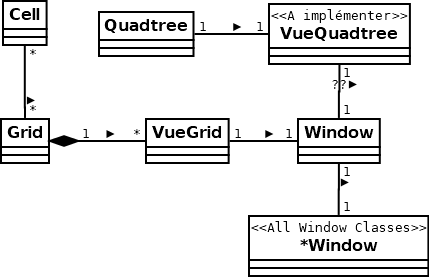
\includegraphics[width=0.5\textwidth]{images/diagramme.png}
				\caption{Diagramme de classe du projet}
			\end{figure}
			\emph{All Window Classes} fait référence à différentes classes qui héritent de \textbf{JDialog} et qui permettent de générer une nouvelle fenêtre dans laquelle on peut configurer certains paramètres.
		
		\subsection{Interface graphique} \label{interface}
			Pour concevoir l'interface graphique nous avons utilisé le principe Modèle-Vue-Contrôleur étudié dans l'unité d'enseignement "Interfaces Graphiques et Design Patterns".\\
			Les packages utilisés ont notamment été \textbf{javax.swing} pour les éléments graphiques et \textbf{java.awt.event} pour la gestion des événements sur l'interface.
			\newpage
			
			\begin{figure}[!h]
				\noindent
				\makebox[\textwidth]{
					\begin{tikzpicture}
						\node[anchor=north west,inner sep=0] (interface) at (0,0) {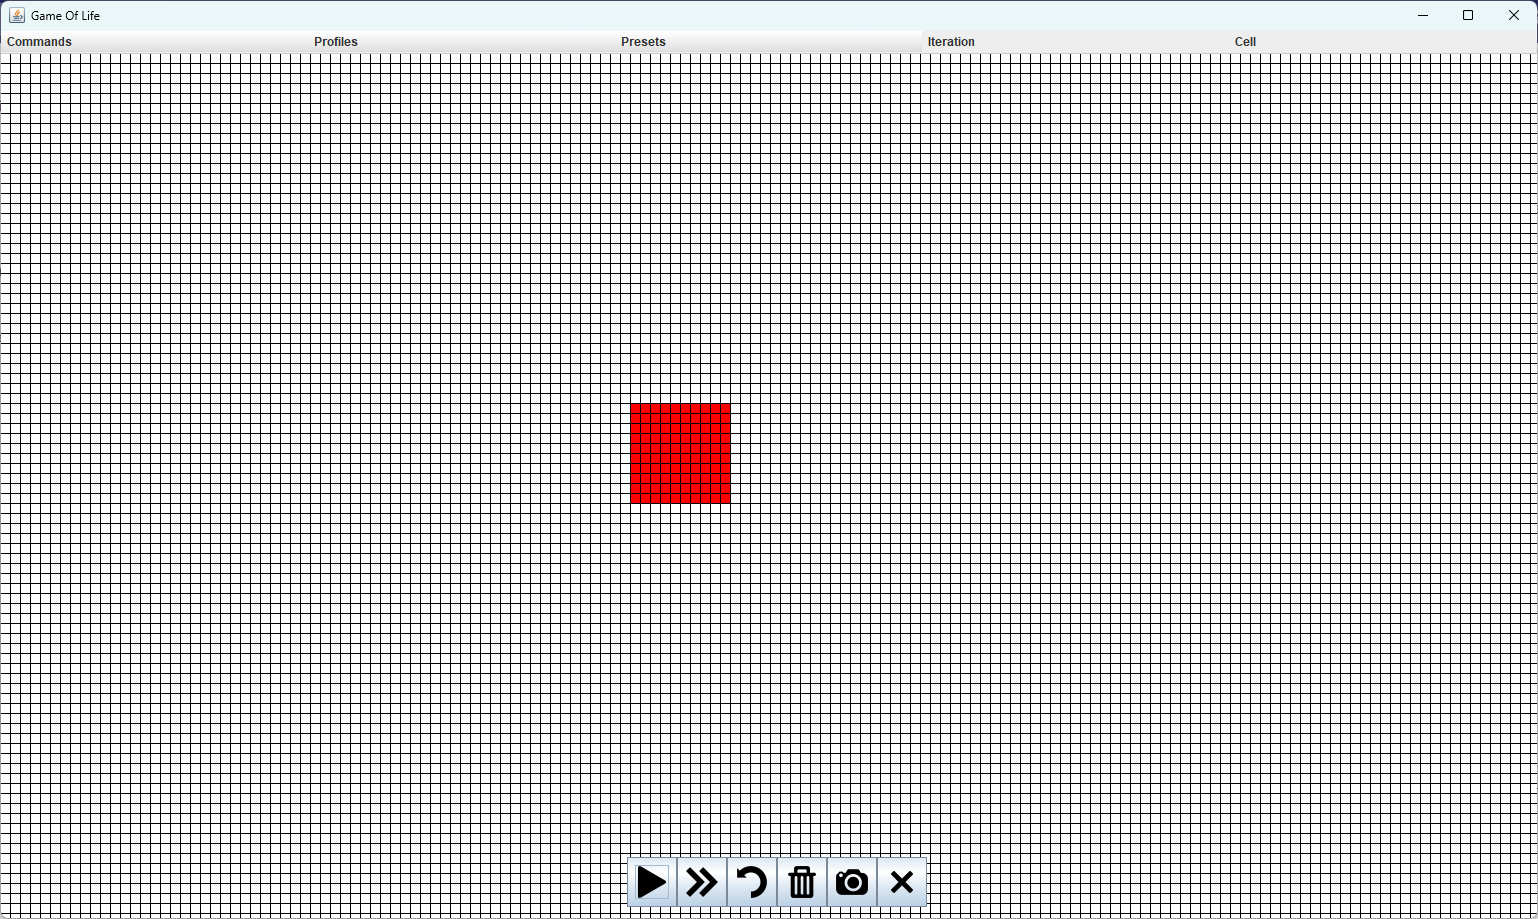
\includegraphics[width=1.5\textwidth, center]{images/interface.jpg}};
						
						\node[fit={(-3.5,0) (17.25,-1)}, inner sep=0pt, draw=blue, line width= 2] (menurect) {};
						\node[] (menu) at (6.875, 0.5){Menu};
						
						\node[fit={(4.75,-11.25) (9.25,-12.25)}, inner sep=0pt, draw=blue, line width= 2] (raccourcirect) {};
						\node[] (raccourci) at (7, -13){Raccourcis};
						
						\node[fit={(4.85,-5.25) (6.50,-6.85)}, inner sep=0pt, draw=blue, line width= 2] (cellrect) {};
						\node[] (cell) at (0, -13){Carré de cellules vivantes};
						\draw[ultra thick,->, blue] (cell) to (cellrect) ;
						
						\node[] (vuegrid) at (15, -13){Vue de la grille};
						\draw[ultra thick,->, blue] (vuegrid) to (12, -6.5) ;

				\end{tikzpicture}}
				\caption{Capture d'écran de l'interface graphique}
			\end{figure}
			\newpage
			L'interface est donc composée de deux éléments principaux à savoir le menu et la vue de la grille.\\ 
			Le menu contient 5 onglets : \\
			\begin{itemize}[label= ]
				\item \textbf{Commands} : Pour les différentes actions (aussi accessibles par les raccourcis).
				\item \textbf{Profiles} : Permet de charger, sauvegarder et supprimer des profiles.
				\item \textbf{Presets} : Permet de charger, sauvegarder et supprimer des modèles prédéfinis de grille.
				\item  \textbf{Iteration} : Pour modifier les paramètres de simulation.
				\item \textbf{Cell} : Pour modifier les paramètres des cellules de la grille.
			\end{itemize}
			
			Lorsque l’on souhaite modifier les paramètres de la simulation, la fenêtre ci-dessous apparaît :
			\begin{figure}[!ht]
				\centering
				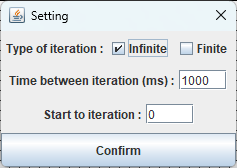
\includegraphics[width=.5\textwidth]{images/jdialog.png}
				\caption{fenêtre - configuration de la simulation}
			\end{figure}\\
		
			L’utilisateur peut alors modifier les paramètres de la simulation et les confirmer. A cette étape, nous avons dû implémenter Threads car lorsqu’une simulation était exécutée et que l’on souhaitait cliquer sur un bouton, les ressources étaient occupées par la simulation ne laissant plus de place pour l’exécution des actions du bouton.
			
			
			\subsection{Éléments techniques}
			\subsubsection{HashLife} \label{hashlife}
			Hashlife est un algorithme créé par Bill Gosper dans les années 1980 pour améliorer la vitesse de calcul des motifs du Jeu de la vie. Hashlife utilise des tables de hachage, lui permettant de calculer des figures très compliquées très rapidement.
			
			Nous avons implémenté l’algorithme HashLife avec des quadtrees, il fonctionne et nous donne des résultats de calculs nettement supérieurs à ceux d’une grille. Cependant, la complexité des quadtree nous a freiné dans l’implémentation de HashLife sur la partie graphique. En effet, les fonctions pour afficher une partie de la grille, (dé)zoomer et se déplacer sur la grille étant complexes avec les quadtrees, nous avons fait le choix d’implémenter les fonctionnalités souhaitées avec les grilles, et de laisser HashLife sur le côté. Le temps nous manquant, la simulation du Jeu de la vie se fait sur un automate cellulaire dans l’interface graphique.
			
			
			\subsubsection{Ant}
			Pour nous aider dans la réalisation du projet, nous avons utilisé apache Ant, un utilitaire de scripts (principalement pour les projets en Java) qui permet de faire de manière simple des tâches répétitives qui deviennent compliquées au fur et à mesure que le projet grandit. Nous avons créé 8 scripts permettant de simplifier les manipulations sur le projet. Pouvoir compiler, exécuter et nettoyer le projet à partir d'une simple commande nous a permis de gagner du temps et nous a évité bien des erreurs dans les commandes;
			\begin{table}[!htpb]
				\center
				\begin{tabular}{|l|l|}
					\hline
					\textbf{Nom Commande} & \textbf{Description commande} \\
					\hline
					clean & supprime le dossier bin \\
					\hline
					init & crée les repertoires bin, doc et dist \\
					\hline
					compile & compile le projet \\
					\hline
					run & lance l'application \\
					\hline
					test & lance les tests \\
					\hline
					doc & génère la documentation \\
					\hline
					build & construit le projet (compile + doc + .jar + clean) \\
					\hline
				\end{tabular}
				\caption{Commandes ant}
				\label{tab1}
			\end{table}
			
			\subsubsection{Threads}
			Pour pouvoir mettre pause nous avons dû recourir à l’utilisation de threads. L’usage de ceux-ci était nécessaire car exécuter la génération des cellules dans le thread principale monopolisait le processeur. Pour remédier à cela nous avons du implémenter l’interface Runnable dans Window. Grâce à la fonction run() de Runnable, nous exécutons la génération des cellules dans un autre thread, ce qui permet à la page de reste opérationnelle. 
			
			\subsubsection{Extension .gol} \label{config}
			Afin de rendre le chargement et la sauvegarde des profils et des modèles prédéfinis plus simple, nous avons implémenté le type .gol, pour les profils, les fichiers sont du type nom.gol.profile, permettant de savoir comment les données doivent être chargées. Les fichiers pour les modèles prédéfinis fonctionnent de la même manière : name.gol.preset.\\
			
			Les profils et les modèles prédéfinis sont sauvegardés de la manière suivante :
			\begin{figure}[!ht]
				\centering
				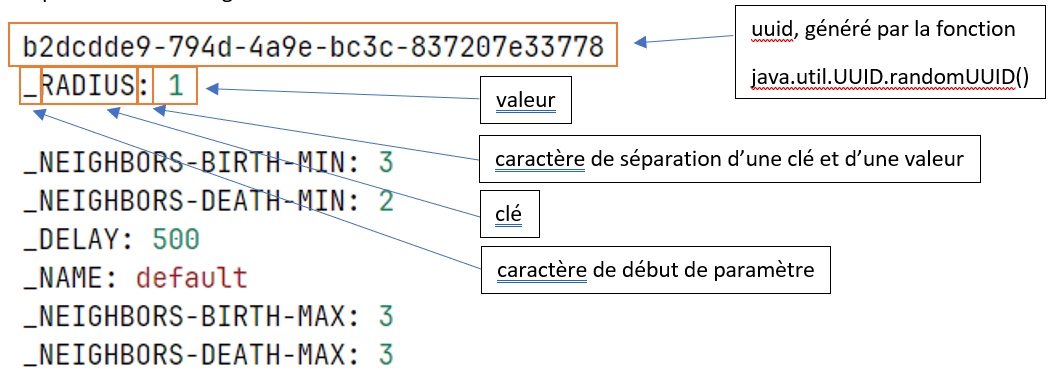
\includegraphics[width=\textwidth]{images/profiles.png}
				\caption{fichier - profiles.gol.profile}
			\end{figure}\\
			\begin{figure}[!ht]
				\centering
				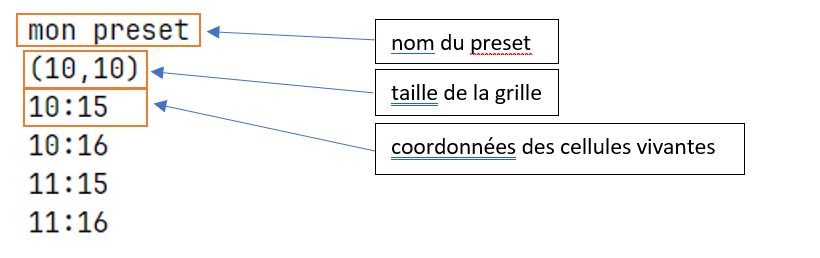
\includegraphics[width=\textwidth]{images/presets.png}
				\caption{fichier - presets.gol.preset}
			\end{figure}
			
			Pour éviter les conflits et les suppressions de fichiers, les profils et les modèles prédéfinis sont chargés sur des fichier profiles.gol.profile et presets.gol.preset dans les fichiers de l’application. Ils ne sont donc pas accessibles par l’utilisateur.
			
			\section{Tests} \label{tests}
			Pour s’assurer que les fonctions écrites et utilisées fonctionnent, nous avons mis en place une partie pour les tests dans laquelle nous testons toutes les fonctions de tous les fichiers du projet. Permettant ainsi d’éviter certaines erreurs lors de l’utilisation des fonctions du projet.
			
			Les tests ont permis d'identifier et de corriger rapidement les erreurs qui peuvent survenir lors de l'exécution de certaines fonctions, mais ils permettent également de modifier ces fonctions pour les rendre plus génériques.
			
			De plus, l'utilisation de la surcharge sur des fonctions spécifiques en s'adaptant à des paramètres spécifiques a permis de faciliter les tests.
			
			Ci-dessous le résultat obtenu avec la commande ant test, qui exécute tous les tests
			\begin{figure}[!h]
				\centering
				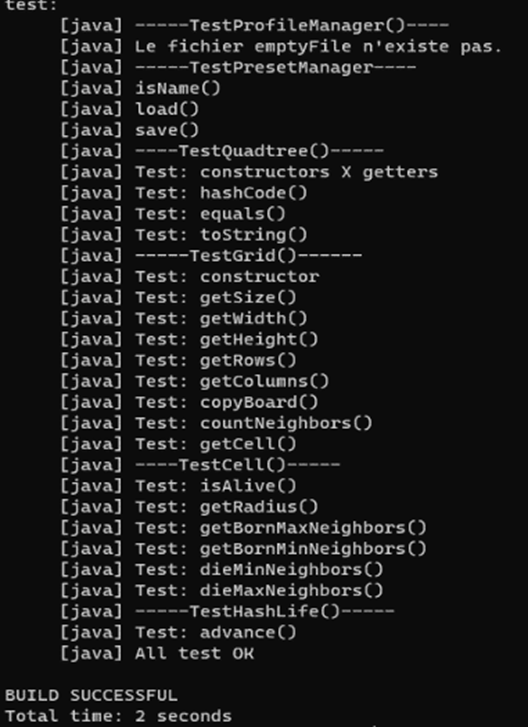
\includegraphics{images/tests.png}
				\caption{Capture d'écran de l'exécution des tests}
			\end{figure}
			\newpage
			
			\section{Conclusion}
			\subsection{Les améliorations possibles}
			Malgré une cohésion de groupe assez bonne, notre mauvaise connaissance de certains outils tels que git nous a parfois fait faire des erreurs que l’on ne devrait pas faire, telles que : des messages de commit pas clairs, push une version qui ne fonctionne pas, ne pas faire relire son code aux autres, ne pas tester son code …
			
			Nous n’avons aussi pas eu le temps d’implémenter la vue pour les quadtree, ne permettant donc pas l’utilisation de l’algorithme HashLife malgré son implémentation. La conception de l’application est une conception commune que l’on retrouve dans une bonne partie des projets en java, cependant la manière dont nous avons implémenté certaines fonctionnalités pourrait être revue afin d’optimiser l’application. Le code que nous avons fourni est maintenable et peut facilement évoluer dans le temps.
			
			\subsection{Ce que le projet nous a apporté}
			Pour finaliser ce rapport, nous pouvons affirmer que le projet que nous fournissons est maintenable et évolutif. Tous les objectifs que nous nous étions fixés au début n’ont pas été atteints, cependant les idées principales sont implémentées et fonctionnelles. Nous retiendrons de cette expérience que la communication et la planification sont les clés d’un projet réussi.
			

\end{document}